\documentclass[11pt,a4paper]{article}
\usepackage{geometry}
\geometry{top=2.5cm, bottom=2.5cm, left=2.5cm, right=2.5cm}
\usepackage{graphicx}
\usepackage{adjustbox}
\usepackage{setspace}
\usepackage{tikz}
\usetikzlibrary{calc}
\usepackage{eso-pic}
\usepackage{titlesec}
\usepackage{float}
\usepackage{array}
\usepackage{booktabs}
\usepackage{xcolor}
\usepackage{caption}

\usepackage{listings}
\captionsetup[lstlisting]{labelformat=empty}
\lstset{
    language=Verilog,
    basicstyle=\ttfamily\footnotesize,
    keywordstyle=\color{blue}\bfseries,
    identifierstyle=\color{black},
    commentstyle=\color{green!60!black},
    stringstyle=\color{purple},
    showstringspaces=false,
    numbers=left,
    numberstyle=\tiny\color{gray},
    frame=single,
    rulecolor=\color{black!30},
    breaklines=true,
    backgroundcolor=\color{gray!5},
    captionpos=b
}

\titleformat{\section}{\fontsize{18pt}{22pt}\bfseries}{\thesection}{1em}{}
\titleformat{\subsection}{\fontsize{15pt}{19pt}\bfseries}{\thesubsection}{1em}{}

\usepackage{tocloft}
\renewcommand{\cftsecleader}{\cftdotfill{\cftdotsep}}

\usepackage{xepersian}
\settextfont{XB Niloofar}
\setdigitfont{XB Niloofar}

\begin{document}

\AddToShipoutPictureBG{
    \begin{tikzpicture}[remember picture, overlay]
        \node[draw, line width=2.5pt, minimum width=\paperwidth-2cm, minimum height=\paperheight-2cm, inner sep=0pt] at (current page.center) {};
        \node[draw, line width=1.0pt, minimum width=\paperwidth-2.3cm, minimum height=\paperheight-2.3cm, inner sep=0pt] at (current page.center) {};
    \end{tikzpicture}
}

\begin{titlepage}
    \centering
    \vspace*{0.2cm}
    
\includegraphics[width=3.5cm]{images/logo.png} \\[0.4cm] 
    {\fontsize{14pt}{18pt}\selectfont دانشگاه صنعتی شریف} \\[0.2cm]
    {\fontsize{14pt}{18pt}\selectfont دانشکده مهندسی کامپیوتر} \\[0.6cm]
    {\fontsize{18pt}{22pt}\bfseries گزارش کار آزمایش پنجم}

    \vspace{1.2cm}
    {\fontsize{12pt}{16pt}\selectfont عنوان:} \\[0.3cm]
    {\fontsize{22pt}{28pt}\bfseries طراحی ضرب‌کننده} \\[0.3cm]
    
    \vspace{1.0cm}
    {\fontsize{12pt}{16pt}\selectfont نام درس:} \\[0.3cm]
    {\fontsize{14pt}{18pt}\bfseries آزمایشگاه طراحی سامانه‌های رقمی}

    \vspace{1.0cm}
    {\fontsize{12pt}{16pt}\selectfont تابستان ۱۴۰۵}

    \vspace{1.0cm}
    {\fontsize{12pt}{16pt}\selectfont استاد:} \\[0.3cm]
    {\fontsize{14pt}{18pt}\bfseries دکتر اجلالی}
    
    \vspace{0.6cm}
    {\fontsize{12pt}{16pt}\selectfont دستیار استاد:} \\[0.3cm]
    {\fontsize{14pt}{18pt}\bfseries علی اثنی عشری}

\vspace{1.0cm}
{\fontsize{12pt}{16pt}\selectfont گروه ۲\par}
\vspace{0.3cm}
{\fontsize{14pt}{20pt}\bfseries
علی سلطانی - 403106092\\[0.15cm]
یگانه کربلایی - 403106527\\[0.15cm]
محمدمهدی مرادی - 403106681\par}

    \vfill
\end{titlepage}

\newpage
\tableofcontents
\newpage

\section{مقدمه و روش بوث}
روش\LTRfootnote{Algorithm} بوث یکی از روش‌های کارآمد برای ضرب اعداد علامت‌دار یا همان اعداد مکمل دو\LTRfootnote{Two's Complement} در سخت‌افزار است. در روش ضرب معمولی، وجود اعداد منفی نیازمند پیش‌پردازش است، اما روش بوث با بررسی همزمان دو بیت متوالی از ضریب، عملیات ضرب را بدون نیاز به تغییر علامت اعداد به درستی انجام می‌دهد.

\subsection{نحوه کارکرد روش پایه}
در این روش ما از چهار ثبات\LTRfootnote{Register} اصلی استفاده می‌کنیم:
\begin{itemize}
    \item \textbf{ثبات $M$:} دربردارنده عدد مضروب\LTRfootnote{Multiplicand}.
    \item \textbf{ثبات $Q$:} دربردارنده عدد ضریب\LTRfootnote{Multiplier}.
    \item \textbf{ثبات $A$:} ثبات انباشتگر\LTRfootnote{Accumulator} که در ابتدا مقدار صفر دارد.
    \item \textbf{بیت $Q_{-1}$:} یک بیت کمکی که در ابتدا صفر است.
\end{itemize}

در هر مرحله، دو بیت $Q_0$ (بیت دارای کمترین ارزش ضریب) و $Q_{-1}$ بررسی می‌شوند:
\begin{itemize}
    \item اگر مقادیر برابر با $00$ یا $11$ باشند: ترکیب ۹ بیتی $A Q Q_{-1}$ به صورت یکپارچه به اندازه یک بیت به سمت راست شیفت حسابی\LTRfootnote{Arithmetic Shift Right} داده می‌شود.
    \item اگر مقادیر برابر با $01$ باشند: ابتدا مقدار $M$ با $A$ جمع می‌شود ($A = A + M$) و سپس ترکیب ۹ بیتی $A Q Q_{-1}$ به سمت راست شیفت داده می‌شود.
    \item اگر مقادیر برابر با $10$ باشند: مقدار $M$ از $A$ تفریق می‌شود ($A = A - M$) و سپس ترکیب ۹ بیتی $A Q Q_{-1}$ به سمت راست شیفت داده می‌شود.
\end{itemize}

\subsection{مثال روش پایه\LTRfootnote{Standard}: ضرب عدد $7$ در $3$}
در این مثال ۴ بیتی، فرض می‌کنیم $M = 0111$ (عدد $7$) و $Q = 0011$ (عدد $3$) است.
بنابراین مقدار مکمل آن، یعنی $-M = 1001$ خواهد بود. زمان اجرای این روش همواره برابر با تعداد بیت‌ها است؛ یعنی برای اعداد ۴ بیتی دقیقاً ۴ چرخه ساعت نیاز است.

\begin{table}[H]
    \centering
    \begin{adjustbox}{max width=\textwidth}
    \begin{tabular}{|c|c|c|c|c|l|}
        \hline
        \textbf{مرحله} & \textbf{$Q_0 Q_{-1}$} & \textbf{$Q_{-1}$} & \textbf{Q} & \textbf{A} & \textbf{اقدام بعدی} \\
        \hline
        0 & 10 & 0 & 0011 & 0000 & وضعیت $10$ $\leftarrow$ تفریق و سپس شیفت \\
        \hline
        1 & 11 & 1 & 1001 & 1100 & وضعیت $11$ $\leftarrow$ فقط شیفت \\
        \hline
        2 & 01 & 1 & 0100 & 1110 & وضعیت $01$ $\leftarrow$ جمع و سپس شیفت \\
        \hline
        3 & 00 & 0 & 1010 & 0010 & وضعیت $00$ $\leftarrow$ فقط شیفت \\
        \hline
        4 & - & 0 & 0101 & 0001 & پایان عملیات \\
        \hline
    \end{tabular}
    \end{adjustbox}
    \caption{مراحل ضرب $7 \times 3$ با استفاده از روش پایه}
\end{table}
جواب نهایی از ترکیب ثبات‌های $A$ و $Q$ به دست می‌آید: $00010101$ که در مبنای ده‌دهی برابر با عدد $21$ می‌باشد.

\newpage
\section{روش بوث بهینه‌شده}
در روش پایه، در صورتی که با بلوکی از صفرهای متوالی یا یک‌های متوالی در ضریب مواجه شویم، سیستم تنها عملیات شیفت یک‌بیتی را تکرار می‌کند. در معماری بهینه‌شده این آزمایش، سیستم به جای بررسی مرزهای تک‌بیتی، کل بلوک‌های صفر و یک متوالی در ثبات $Q$ را شناسایی کرده و در یک چرخه ساعت از روی آن‌ها پرش می‌کند. زمان اجرای روش بهینه‌شده به جای مقدار ثابت $N$ چرخه، برابر با تعداد بلوک‌های متوالی در ضریب است که همواره کمتر یا مساوی روش پایه خواهد بود.

در این معماری برای تسریع عملیات، به جای آنکه ثبات نتیجه نهایی (\lr{result}) در هر گام به سمت راست شیفت بخورد (که رویکرد روش پایه است)، این ثبات کاملاً در جای خود ثابت نگه داشته می‌شود. در عوض، برای حفظ ارزش مکانیِ اعداد در هنگام جمع و تفریق، خودِ مقدار مضروب (\lr{M}) پیش از ورود به محاسبات، به تعداد پرش‌های انجام‌شده تا آن لحظه، به سمت چپ شیفت داده می‌شود. همچنین از آنجایی که ثبات نتیجه نهایی هشت بیتی است، مضروب چهار بیتی باید در یک متغیر میانی بسط علامت یابد تا با ثبات نتیجه قابل جمع باشد. برای پیاده‌سازی این منطق و تشخیص اینکه در هر گام چه تعداد کلاک باید پرش شود، از مدارهای ترکیبی بهره گرفته شده است که متغیرهای آن در ادامه معرفی شده‌اند.

\subsection{متغیرها و منطق پیاده‌سازی}
در این معماری، مدار در هر چرخه کلاک به بیت اول ضریب فعلی (بیت دارای کمترین ارزش مکانی) نگاه می‌کند و بر اساس آن تصمیم‌گیری می‌نماید:
\begin{itemize}
    \item \textbf{تشخیص بلوک ۱ و تفریق:} اگر بیت اول برابر با $1$ باشد، به معنای رسیدن به بلوکی از یک‌های متوالی است. مدار عمل تفریق را انجام داده و سپس عملیات پرش را اجرا می‌کند.
    \item \textbf{تشخیص بلوک ۰ و جمع:} اگر بیت اول برابر با $0$ باشد، به معنای رسیدن به بلوکی از صفرهای متوالی است. مدار عمل جمع را انجام داده و سپس عملیات پرش را اجرا می‌کند.
    \item \textbf{مبنای پرش:} مبنای پرش در این روش، شمارش تعداد بیت‌های مشابه و متوالی در سمت راست ضریب است. با محاسبه تفاضل جایگاه اولین بیتِ یک و اولین بیتِ صفر، مدار دقیقاً متوجه می‌شود که چند چرخه بی‌حاصل را باید در یک گام پشت سر بگذارد.
\end{itemize}

برای اجرای دقیق این عملیات بدون از دست رفتن ارزش مکانی\LTRfootnote{Place Value} اعداد، از متغیرهای زیر استفاده شده است:
\begin{itemize}
    \item \textbf{\lr{shift\_Q}:} تعداد بیت‌هایی که در چرخه فعلی باید از روی آن‌ها در ضریب پرش شود (همان مبنای پرش).
    \item \textbf{\lr{shift\_M}:} مجموع کل پرش‌های انجام‌شده تا این لحظه. این متغیر ارزش مکانی مضروب را تنظیم می‌کند.
    \item \textbf{\lr{op}:} نوع عملیات را تعیین می‌کند (صفر برای جمع، یک برای تفریق).
    \item \textbf{\lr{valid}:} در صورتی که ضریب با بلوک صفر آغاز شود، این سیگنال صفر می‌شود تا از اجرای جمع با صفر جلوگیری کند. این متغیر در واقع نشان‌دهنده این است که آیا در چرخه فعلی، عملیات محاسباتی (جمع یا تفریق) نیز داریم، یا اینکه سیستم فقط باید عمل شیفت را انجام دهد.
    \item \textbf{\lr{result}:} ثبات دربرگیرنده نتیجه نهایی که برخلاف روش پایه ثابت است و شیفت نمی‌خورد. در عوض، مقدار مضروب پیش از محاسبات به اندازه \lr{shift\_M} به چپ شیفت داده می‌شود.
\end{itemize}

\subsection{مثال روش بهینه‌شده: ضرب عدد $7$ در $3$}
ورودی‌ها: $M = 0111$ و $Q = 0011$. 
\begin{table}[H]
    \centering
    \begin{adjustbox}{max width=\textwidth}
    \begin{tabular}{|c|c|c|c|c|c|l|c|}
        \hline
        \textbf{ساعت} & \textbf{Q فعلی} & \textbf{valid} & \textbf{op} & \textbf{shift-Q} & \textbf{shift-M} & \textbf{اقدام بعدی} & \textbf{result} \\
        \hline
        0 & 0011 & - & - & - & 0 & - & $0$ \\
        \hline
        1 & 0011 & 1 & 1 & 2 & 0 & بیت اول $1$ است $\leftarrow$ تفریق و شیفت $Q$ به اندازه ۲ & $0 - (M \ll 0) = -7$ \\
        \hline
        2 & 00 & 1 & 0 & 2 & 2 & بیت اول $0$ است $\leftarrow$ جمع و شیفت $Q$ به اندازه ۲ & $-7 + (M \ll 2) = 21$ \\
        \hline
        3 & - & - & - & - & 4 & اتمام & \textbf{21} \\
        \hline
    \end{tabular}
    \end{adjustbox}
    \caption{مراحل ضرب $7 \times 3$ با روش بهینه‌شده}
\end{table}
عملیات به جای چهار چرخه، در دو چرخه به اتمام رسید و متغیر \lr{shift\_M} به مقدار $4$ رسید که نشان‌دهنده پایان کار است.

\newpage
\section{پیاده‌سازی سخت‌افزاری و بررسی کدها}
در این بخش، معماری مدار به دو بخش کلی \textbf{واحد کنترل}\LTRfootnote{Control Unit} و \textbf{مسیر داده}\LTRfootnote{Datapath} تفکیک گردیده است. تمامی اجزا در قالب پیمانه‌های\LTRfootnote{Module} مجزا نوشته شده‌اند.

\subsection{پیمانه واحد کنترل}
این پیمانه مغز متفکر مدار است که با بررسی ضریب، دستورات لازم را به مسیر داده ارسال می‌کند.

\begin{LTR}
\begin{lstlisting}[title={\rl{کد پیمانه واحد کنترل}}]
module ControlUnit(
    input clk,
    input rst,
    input [3:0] Q,
    output done,
    output op,
    output valid,
    output [2:0] shift_Q,
    output reg [2:0] shift_M
);

    wire [2:0] first_one;
    wire [2:0] first_zero;

    // Priority encoder logic to find first '1'
    assign first_one = (Q[0] == 1) ? 3'b000 :
                       (Q[1] == 1) ? 3'b001 :
                       (Q[2] == 1) ? 3'b010 :
                       (Q[3] == 1) ? 3'b011 : 3'b100;

    // Priority encoder logic to find first '0'
    assign first_zero = (Q[0] == 0) ? 3'b000 :
                        (Q[1] == 0) ? 3'b001 :
                        (Q[2] == 0) ? 3'b010 :
                        (Q[3] == 0) ? 3'b011 : 3'b100;

    // Determine operation based on LSB
    assign op = (Q[0] == 0) ? 0 : 1; 
    
    // Disable addition if starting with a block of zeros
    assign valid = ~((shift_M == 0) && (Q[0] == 0));

    // Calculate jump size
    assign shift_Q = (Q[0] == 0) ? first_one - first_zero : first_zero - first_one;

    // Accumulate total shifts synchronously
    always @(posedge clk) begin
        if (rst) begin
            shift_M <= 0;
        end else begin
            if (!done) begin
                shift_M <= shift_M + shift_Q;
            end
        end
    end

    // Flag generation when 4 bits are processed
    assign done = (shift_M >= 3'b100) ? 1 : 0;

endmodule
\end{lstlisting}
\end{LTR}

\begin{itemize}
    \item \textbf{خطوط ۲ تا ۴ (ورودی‌ها):} سیگنال ساعت (\verb|clk|)، بازنشانی (\verb|rst|) و وضعیت ۴ بیتیِ فعلیِ ضریب (\verb|Q|) به عنوان ورودی دریافت می‌شوند.
    \item \textbf{خطوط ۵ تا ۹ (خروجی‌ها):} سیگنال پایان عملیات (\verb|done|)، نوع عملگر (\verb|op|)، مجوز محاسبه (\verb|valid|)، میزان پرش در ضریب (\verb|shift_Q|) و متغیر \lr{shift\_M} که مجموع پرش‌های انجام‌شده تا این لحظه را در خود نگه می‌دارد، تعریف شده‌اند.
    \item \textbf{خطوط ۱۲ تا ۲۴:} در این بخش دو سیم داخلی تعریف شده است. مدارهای منطقیِ ترکیبی (شبیه به رمزگذار اولویت‌دار) از راست به چپ ثبات $Q$ را بررسی می‌کنند تا جایگاه (اندیس) اولین بیتِ یک (\verb|first_one|) و اولین بیتِ صفر (\verb|first_zero|) را پیدا کنند.
    \item \textbf{خط ۲۶:} متغیر \verb|op| با بررسی اولین بیت ضریب تعیین می‌شود، اگر صفر باشد عمل جمع (صفر) و اگر یک باشد عمل تفریق (یک) انتخاب می‌گردد.
    \item \textbf{خط ۲۸:} سیگنال \verb|valid| ارزیابی می‌کند که آیا در اولین چرخه (\lr{\texttt{shift\_M == 0}}) قرار داریم و عدد نیز با صفر شروع شده است یا خیر. این سیگنال مشخص می‌کند که آیا در این کلاک به محاسبات حسابی (جمع و تفریق) نیاز داریم، یا اینکه مدار فقط باید عملیات شیفت را انجام دهد.
    \item \textbf{خط ۳۰:} مقدار پرش (\verb|shift_Q|) از طریق تفاضل اندیس اولین صفر و اولین یک به دست می‌آید که سبب عبور یک‌باره از روی بلوک‌های تکراری می‌شود.
    \item \textbf{خطوط ۳۲ تا ۴۰:} این بلوک همگام با ساعت عمل می‌کند. در صورت فعال بودن \verb|rst|، مقدارِ \verb|shift_M| صفر می‌شود و در غیر این صورت، در هر چرخه مقدار پرش جدید (\verb|shift_Q|) به مقدار مجموع پرش‌های قبلیِ \verb|shift_M| افزوده می‌شود تا ارزش مکانی عدد برای محاسبات بعدی حفظ گردد.
    \item \textbf{خط ۴۲:} سیگنال \verb|done| بررسی می‌کند که آیا مجموع شیفت‌ها به عدد ۴ (اندازه بیت‌های ورودی) رسیده است یا خیر.
\end{itemize}

\subsection{پیمانه مسیر داده}
این پیمانه فاقد تصمیم‌گیری منطقی بوده و صرفاً وظیفه اجرای محاسبات ریاضی و عملیات شیفت‌دهی را بر عهده دارد.

\begin{LTR}
\begin{lstlisting}[title={\rl{کد پیمانه مسیر داده}}]
module Datapath(
    input clk,
    input rst,
    input done,
    input op,
    input valid, 
    input [2:0] shift_Q,
    input [2:0] shift_M,
    input [3:0] M,
    input [3:0] Q_in,
    output reg [7:0] result,
    output reg [3:0] Q_out
);

    reg [7:0] M_extended;        // Sign-extended multiplicand

    always @(posedge clk) begin
        if (rst) begin
            // Reset conditions
            result <= 8'b0;
            Q_out <= Q_in;
            M_extended <= {{4{M[3]}}, M}; // Sign extension to 8 bits
        end else begin
            if (!done) begin
                // Shift multiplier logic right
                Q_out <= Q_out >> shift_Q;
                
                // Arithmetic operation block
                if (valid) begin
                    if (op == 0) begin
                        result <= result + (M_extended << shift_M);
                    end else begin
                        result <= result - (M_extended << shift_M);
                    end
                end
            end
        end
    end

endmodule
\end{lstlisting}
\end{LTR}

\begin{itemize}
    \item \textbf{خطوط ۲ تا ۱۰ (ورودی‌ها):} علاوه بر ساعت و بازنشانی، این پیمانه مضروب (\verb|M|) و ضریب اولیه (\verb|Q_in|) را از کاربر و تمامی فرمان‌های صادرشده (\verb|done, op, valid, shift_Q, shift_M|) را از واحد کنترل دریافت می‌کند.
    \item \textbf{خطوط ۱۱ تا ۱۲ (خروجی‌ها):} ثبات ۸ بیتی \verb|result| برای نگهداری جواب نهایی و ثبات \verb|Q_out| برای ارسال باقیمانده‌ی ضریب به واحد کنترل در نظر گرفته شده‌اند.
    \item \textbf{خط ۱۵:} یک ثبات میانی ۸ بیتی به نام \verb|M_extended| جهت انجام عمل بسط علامت تعریف شده است. از آنجا که این مقدار باید با ثبات نتیجه (\verb|result|) که هشت بیتی است جمع یا تفریق شود، لازم است \verb|M| نیز پیش از محاسبه به هشت بیت گسترش یابد تا مدار دچار سرریز\LTRfootnote{Overflow} نگردد.
    \item \textbf{خطوط ۱۸ تا ۲۱:} در صورت فعال شدن \verb|rst|، جواب نهایی صفر شده، ضریب اولیه در ثبات وضعیت قرار می‌گیرد و از همه مهم‌تر، متغیر ۴ بیتیِ $M$ با کپی کردن بیتِ ارزش مکانیِ علامت، به یک قالب ۸ بیتی (\verb|M_extended|) گسترش می‌یابد.
    \item \textbf{خط ۲۴:} در وضعیت کار عادی، ثبات ضریب به اندازه \verb|shift_Q| به راست شیفت حسابی داده می‌شود تا بیت‌های پردازش‌شده دور ریخته شوند.
    \item \textbf{خطوط ۲۶ تا ۳۲:} در صورت دریافت مجوز (\verb|valid|)، با توجه به نوع عملگر (\verb|op|)، مقدار بسط‌یافته‌ی مضروب ابتدا به میزان \verb|shift_M| به چپ شیفت داده شده (جهت تنظیم ارزش مکانی) و سپس با ثبات \verb|result| جمع یا از آن تفریق می‌گردد.
\end{itemize}

\subsection{پیمانه سطح بالا}
این پیمانه نقش سیم‌کشی و اتصال دو بخش پیشین را بر عهده دارد.

\begin{LTR}
\begin{lstlisting}[title={\rl{کد پیمانه سطح بالا}}]
module Top(
    input clk,
    input rst,
    input [3:0] M,
    input [3:0] Q_in,
    output done,
    output [7:0] result
);

    // Internal wires for interconnection
    wire [2:0] shift_Q;
    wire [2:0] shift_M;
    wire op;
    wire valid; 
    wire [3:0] Q_wire;  

    // Instantiate Control Unit
    ControlUnit control_unit (
        .clk(clk),
        .rst(rst),
        .Q(Q_wire),
        .done(done),
        .op(op),
        .valid(valid),
        .shift_Q(shift_Q),
        .shift_M(shift_M)
    );

    // Instantiate Datapath
    Datapath datapath (
        .clk(clk),
        .rst(rst),
        .done(done),
        .op(op),
        .valid(valid),
        .shift_Q(shift_Q),
        .shift_M(shift_M),
        .M(M),
        .Q_in(Q_in),
        .result(result),
        .Q_out(Q_wire) 
    );
    
endmodule
\end{lstlisting}
\end{LTR}

\begin{itemize}
    \item \textbf{خطوط ۲ تا ۷:} درگاه‌های\LTRfootnote{Ports} اصلی ارتباط مدار با کاربر نهایی تعریف شده‌اند که تنها شامل ورودی‌های اصلی، ساعت، بازنشانی و خروجی‌های نهایی (\verb|result| و \verb|done|) هستند.
    \item \textbf{خطوط ۱۰ تا ۱۴:} سیم‌های واسط (\verb|wire|) برای اتصال درگاه‌های داخلیِ واحد کنترل و مسیر داده به یکدیگر تعریف شده‌اند تا انتقال فرمان‌ها درون‌سیستمی باقی بماند.
    \item \textbf{خطوط ۱۶ تا ۲۵:} پیمانه \verb|ControlUnit| فراخوانی شده و پورت‌های آن به سیم‌های واسط متصل می‌گردند. ورودی \verb|Q| در این بخش از طریق سیم \verb|Q_wire| مستقیماً به خروجی مسیر داده\LTRfootnote{Datapath} متصل است.
    \item \textbf{خطوط ۲۷ تا ۳۹:} پیمانه \verb|Datapath| فراخوانی شده و درگاه‌های آن تنظیم می‌گردند. خروجی \verb|Q_out| در این بخش، اطلاعات لحظه‌ای ضریب را بر روی سیم \verb|Q_wire| قرار می‌دهد تا واحد کنترل در هر لحظه توانایی خواندن آن را داشته باشد.
\end{itemize}

\newpage
\section{آزمایش و میزآزمون}
برای بررسی صحت عملکرد مدار، یک میزآزمون\LTRfootnote{Testbench} تدوین گردید. این بستر مقادیر مختلفی شامل اعداد مثبت، منفی و صفر را شبیه‌سازی می‌کند.

\begin{LTR}
\begin{lstlisting}[title={\rl{کد پیمانه میزآزمون}}]
module tb;
    reg clk;
    reg rst;
    reg signed [3:0] M;
    reg signed [3:0] Q_in;
    wire done;
    wire signed [7:0] result;

    // Instantiate Top Module
    Top uut (
        .clk(clk),
        .rst(rst),
        .M(M),
        .Q_in(Q_in),
        .done(done),
        .result(result)
    );

    // Clock Generation
    always #5 clk = ~clk;

    initial begin
        clk = 0;
        
        // Test Case 1: M=7, Q_in=5, result=35
        rst = 1;
        M = 7;
        Q_in = 5;
        #10;
        rst = 0;
        wait (done);
        #20;

        // Test Case 2: M=-4, Q_in=-6, result=24
        rst = 1;
        M = -4;
        Q_in = -6;
        #10;
        rst = 0;
        wait (done);
        #20;

        // Test Case 3: M=7, Q_in=-3, result=-21
        rst = 1;
        M = 7;
        Q_in = -3;
        #10;
        rst = 0;
        wait (done);
        #20;

        // Test Case 4: M=-5, Q_in=3, result=-15
        rst = 1;
        M = -5;
        Q_in = 3;
        #10;
        rst = 0;
        wait (done);
        #20;

        // Test Case 5: M=0, Q_in=-7, result=0
        rst = 1;
        M = 0;
        Q_in = -7;
        #10;
        rst = 0;
        wait (done);
        #20;

        // Test Case 6: M=-8, Q_in=7, result=-56
        rst = 1;
        M = -8;
        Q_in = 7;
        #10;
        rst = 0;
        wait (done);
        #20;

        // Test Case 7: M=5, Q_in=-1, result=-5
        rst = 1;
        M = 5;
        Q_in = -1;
        #10;
        rst = 0;
        wait (done);
        #20;

        $stop;
    end
endmodule
\end{lstlisting}
\end{LTR}

\subsection{تحلیل موارد آزمون}
در ادامه هر هفت مورد آزمون\LTRfootnote{Test Case} تعریف‌شده بررسی می‌گردد.

\subsubsection{مورد آزمون نخست: ضرب عدد $7$ در $5$}
ورودی‌ها: $M = 0111$ (عدد $7$) و $Q = 0101$ (عدد $5$).
\begin{table}[H]
    \centering
    \begin{adjustbox}{max width=\textwidth}
    \begin{tabular}{|c|c|c|c|c|c|c|c|}
        \hline
        \textbf{ساعت} & \textbf{Q فعلی} & \textbf{valid} & \textbf{op} & \textbf{\lr{shift\_Q}} & \textbf{\lr{shift\_M}} & \textbf{عملیات} & \textbf{result} \\
        \hline
        1 & 0101 & 1 & 1 & 1 & 0 & تفریق & $0 - (7 \ll 0) = -7$ \\
        \hline
        2 & 010 & 1 & 0 & 1 & 1 & جمع & $-7 + (7 \ll 1) = 7$ \\
        \hline
        3 & 01 & 1 & 1 & 1 & 2 & تفریق & $7 - (7 \ll 2) = -21$ \\
        \hline
        4 & 0 & 1 & 0 & 1 & 3 & جمع & $-21 + (7 \ll 3) = 35$ \\
        \hline
        5 & - & - & - & - & 4 & اتمام & \textbf{35} \\
        \hline
    \end{tabular}
    \end{adjustbox}
\end{table}

\begin{figure}[H]
    \centering
    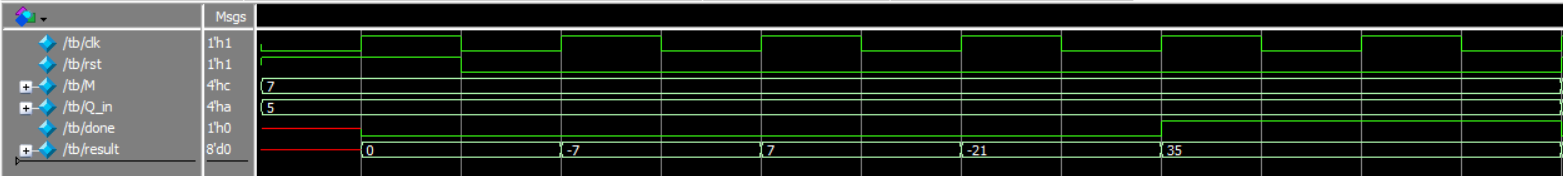
\includegraphics[width=0.9\textwidth]{images/test_case_1.png}
    \caption{شکل‌موج مربوط به مورد آزمون نخست}
\end{figure}

\subsubsection{مورد آزمون دوم: ضرب عدد $-4$ در $-6$}
ورودی‌ها: $M = 1100$ (عدد $-4$) و $Q = 1010$ (عدد $-6$). 
\begin{table}[H]
    \centering
    \begin{adjustbox}{max width=\textwidth}
    \begin{tabular}{|c|c|c|c|c|c|c|c|}
        \hline
        \textbf{ساعت} & \textbf{Q فعلی} & \textbf{valid} & \textbf{op} & \textbf{\lr{shift\_Q}} & \textbf{\lr{shift\_M}} & \textbf{عملیات} & \textbf{result} \\
        \hline
        1 & 1010 & 0 & - & 1 & 0 & - & 0 \\
        \hline
        2 & 101 & 1 & 1 & 1 & 1 & تفریق & $0 - (-4 \ll 1) = 8$ \\
        \hline
        3 & 10 & 1 & 0 & 1 & 2 & جمع & $8 + (-4 \ll 2) = -8$ \\
        \hline
        4 & 1 & 1 & 1 & 1 & 3 & تفریق & $-8 - (-4 \ll 3) = 24$ \\
        \hline
        5 & - & - & - & - & 4 & اتمام & \textbf{24} \\
        \hline
    \end{tabular}
    \end{adjustbox}
\end{table}

\begin{figure}[H]
    \centering
    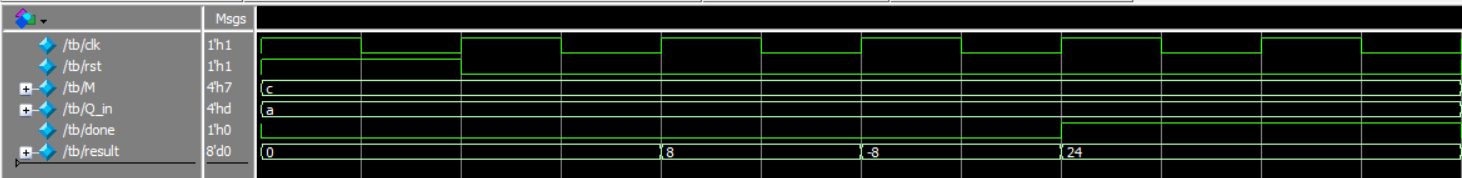
\includegraphics[width=0.9\textwidth]{images/test_case_2.png}
    \caption{شکل‌موج مربوط به مورد آزمون دوم}
\end{figure}

\subsubsection{مورد آزمون سوم: ضرب عدد $7$ در $-3$}
ورودی‌ها: $M = 0111$ (عدد $7$) و $Q = 1101$ (عدد $-3$). 
\begin{table}[H]
    \centering
    \begin{adjustbox}{max width=\textwidth}
    \begin{tabular}{|c|c|c|c|c|c|c|c|}
        \hline
        \textbf{ساعت} & \textbf{Q فعلی} & \textbf{valid} & \textbf{op} & \textbf{\lr{shift\_Q}} & \textbf{\lr{shift\_M}} & \textbf{عملیات} & \textbf{result} \\
        \hline
        1 & 1101 & 1 & 1 & 1 & 0 & تفریق & $0 - (7 \ll 0) = -7$ \\
        \hline
        2 & 110 & 1 & 0 & 1 & 1 & جمع & $-7 + (7 \ll 1) = 7$ \\
        \hline
        3 & 11 & 1 & 1 & 2 & 2 & تفریق & $7 - (7 \ll 2) = -21$ \\
        \hline
        4 & - & - & - & - & 4 & اتمام & \textbf{-21} \\
        \hline
    \end{tabular}
    \end{adjustbox}
\end{table}

\begin{figure}[H]
    \centering
    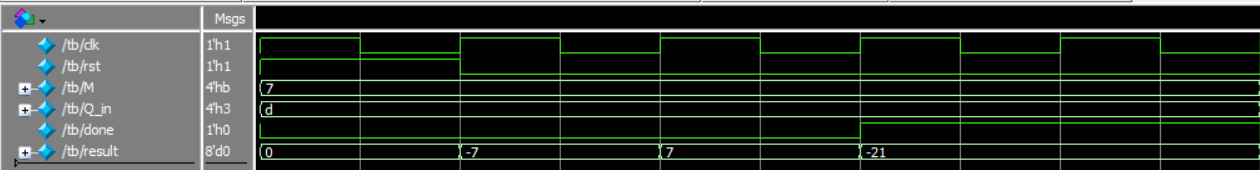
\includegraphics[width=0.9\textwidth]{images/test_case_3.png}
    \caption{شکل‌موج مربوط به مورد آزمون سوم}
\end{figure}

\subsubsection{مورد آزمون چهارم: ضرب عدد $-5$ در $3$}
ورودی‌ها: $M = 1011$ (عدد $-5$) و $Q = 0011$ (عدد $3$).
\begin{table}[H]
    \centering
    \begin{adjustbox}{max width=\textwidth}
    \begin{tabular}{|c|c|c|c|c|c|c|c|}
        \hline
        \textbf{ساعت} & \textbf{Q فعلی} & \textbf{valid} & \textbf{op} & \textbf{\lr{shift\_Q}} & \textbf{\lr{shift\_M}} & \textbf{عملیات} & \textbf{result} \\
        \hline
        1 & 0011 & 1 & 1 & 2 & 0 & تفریق & $0 - (-5 \ll 0) = 5$ \\
        \hline
        2 & 00 & 1 & 0 & 2 & 2 & جمع & $5 + (-5 \ll 2) = -15$ \\
        \hline
        3 & - & - & - & - & 4 & اتمام & \textbf{-15} \\
        \hline
    \end{tabular}
    \end{adjustbox}
\end{table}

\begin{figure}[H]
    \centering
    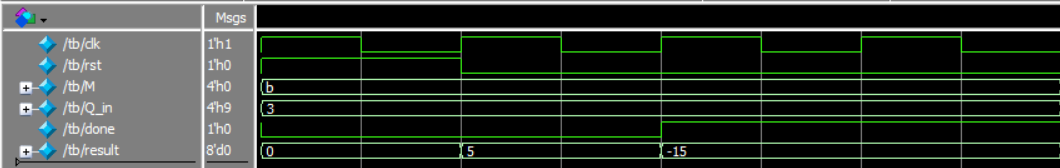
\includegraphics[width=0.9\textwidth]{images/test_case_4.png}
    \caption{شکل‌موج مربوط به مورد آزمون چهارم}
\end{figure}

\subsubsection{مورد آزمون پنجم: ضرب عدد $0$ در $-7$}
ورودی‌ها: $M = 0000$ (عدد $0$) و $Q = 1001$ (عدد $-7$).
\begin{table}[H]
    \centering
    \begin{adjustbox}{max width=\textwidth}
    \begin{tabular}{|c|c|c|c|c|c|c|c|}
        \hline
        \textbf{ساعت} & \textbf{Q فعلی} & \textbf{valid} & \textbf{op} & \textbf{\lr{shift\_Q}} & \textbf{\lr{shift\_M}} & \textbf{عملیات} & \textbf{result} \\
        \hline
        1 & 1001 & 1 & 1 & 1 & 0 & تفریق & $0 - (0) = 0$ \\
        \hline
        2 & 100 & 1 & 0 & 2 & 1 & جمع & $0 + (0) = 0$ \\
        \hline
        3 & 1 & 1 & 1 & 1 & 3 & تفریق & $0 - (0) = 0$ \\
        \hline
        4 & - & - & - & - & 4 & اتمام & \textbf{0} \\
        \hline
    \end{tabular}
    \end{adjustbox}
\end{table}

\begin{figure}[H]
    \centering
    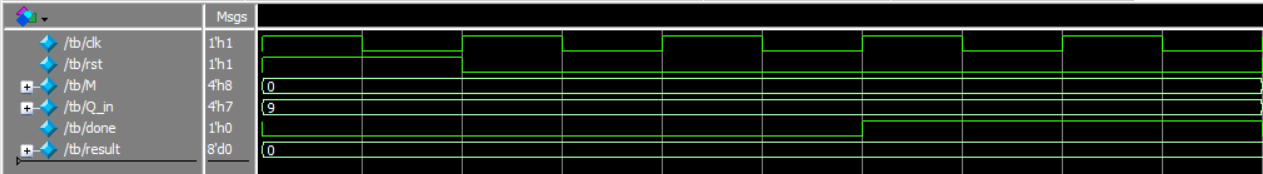
\includegraphics[width=0.9\textwidth]{images/test_case_5.png}
    \caption{شکل‌موج مربوط به مورد آزمون پنجم}
\end{figure}

\subsubsection{مورد آزمون ششم: ضرب عدد $-8$ در $7$}
ورودی‌ها: $M = 1000$ (عدد $-8$) و $Q = 0111$ (عدد $7$).
\begin{table}[H]
    \centering
    \begin{adjustbox}{max width=\textwidth}
    \begin{tabular}{|c|c|c|c|c|c|c|c|}
        \hline
        \textbf{ساعت} & \textbf{Q فعلی} & \textbf{valid} & \textbf{op} & \textbf{\lr{shift\_Q}} & \textbf{\lr{shift\_M}} & \textbf{عملیات} & \textbf{result} \\
        \hline
        1 & 0111 & 1 & 1 & 3 & 0 & تفریق & $0 - (-8 \ll 0) = 8$ \\
        \hline
        2 & 0 & 1 & 0 & 1 & 3 & جمع & $8 + (-8 \ll 3) = -56$ \\
        \hline
        3 & - & - & - & - & 4 & اتمام & \textbf{-56} \\
        \hline
    \end{tabular}
    \end{adjustbox}
\end{table}

\begin{figure}[H]
    \centering
    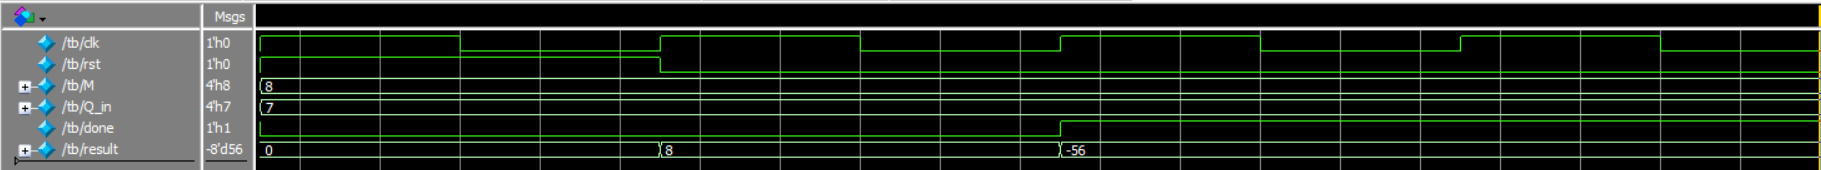
\includegraphics[width=0.9\textwidth]{images/test_case_6.png}
    \caption{شکل‌موج مربوط به مورد آزمون ششم}
\end{figure}

\subsubsection{مورد آزمون هفتم: ضرب عدد $5$ در $-1$}
ورودی‌ها: $M = 0101$ (عدد $5$) و $Q = 1111$ (عدد $-1$).
\begin{table}[H]
    \centering
    \begin{adjustbox}{max width=\textwidth}
    \begin{tabular}{|c|c|c|c|c|c|c|c|}
        \hline
        \textbf{ساعت} & \textbf{Q فعلی} & \textbf{valid} & \textbf{op} & \textbf{\lr{shift\_Q}} & \textbf{\lr{shift\_M}} & \textbf{عملیات} & \textbf{result} \\
        \hline
        1 & 1111 & 1 & 1 & 4 & 0 & تفریق & $0 - (5 \ll 0) = -5$ \\
        \hline
        2 & - & - & - & - & 4 & اتمام & \textbf{-5} \\
        \hline
    \end{tabular}
    \end{adjustbox}
\end{table}

\begin{figure}[H]
    \centering
    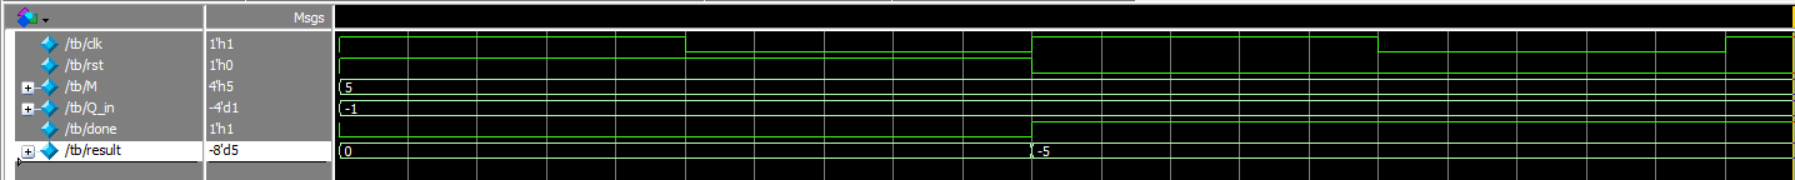
\includegraphics[width=0.9\textwidth]{images/test_case_7.png}
    \caption{شکل‌موج مربوط به مورد آزمون هفتم}
\end{figure}

\newpage
\section{بررسی قابلیت سنتز در نرم‌افزار \lr{Quartus}}
یک پروژه در نرم‌افزار \lr{Quartus} ساخته شد و فایل‌های طراحی به آن افزوده شد. نام پیمانه سطح بالا\LTRfootnote{Top-Level Entity} انتخاب شد. برای بررسی اولیه قابل‌سنتز بودن طراحی، مرحله تحلیل و سنتز از مسیر:
\begin{latin}
\begin{verbatim}
Processing > Start > Start Analysis & Synthesis
\end{verbatim}
\end{latin}
اجرا شد. سپس برای تولید نتایج مرحله تطبیق و امکان مشاهده نمای پس از جایابی، کامپایل کامل از مسیر:
\begin{latin}
\begin{verbatim}
Processing > Start Compilation
\end{verbatim}
\end{latin}
انجام گرفت.

پس از تکمیل کامپایل، سه نمای اصلی از مسیرهای زیر باز شدند:
\begin{latin}
\begin{verbatim}
Tools > Netlist Viewers > RTL Viewer
Tools > Netlist Viewers > Technology Map Viewer (Post-Mapping)
Tools > Netlist Viewers > Technology Map Viewer (Post-Fitting)
\end{verbatim}
\end{latin}

در ادامه، خروجی موفقیت‌آمیز بودن کامپایل و همچنین نماهای بررسی‌شده به ترتیب آورده شده است. نمای سطح انتقال ثبات در واقع یک فهرست اتصالات\LTRfootnote{Netlist} بصری است و نرم‌افزار \lr{Quartus} با تشکیل سلسله‌مراتب\LTRfootnote{Hierarchy} مدار، پروسه را بدون خطا طی کرده است.

\begin{figure}[H]
    \centering
    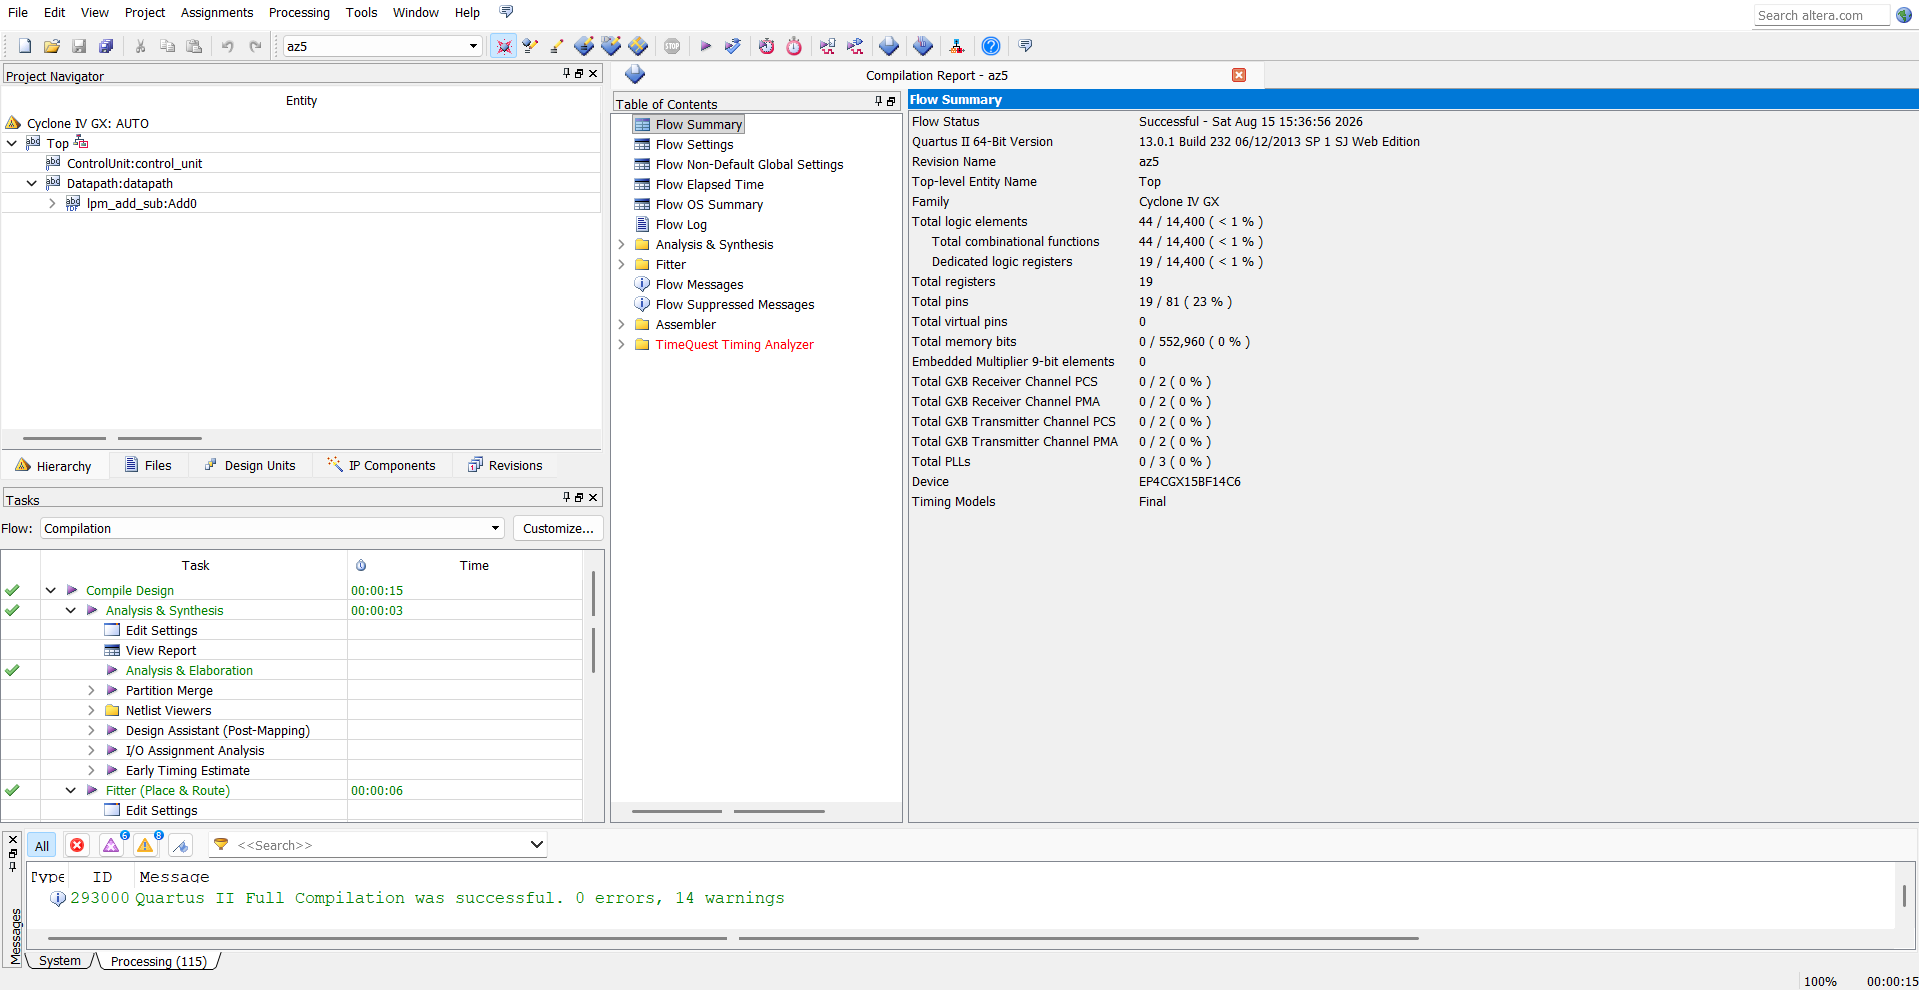
\includegraphics[width=1\textwidth]{images/quartus_compilation.png}
    \caption{گزارش موفقیت‌آمیز بودن کامپایل کامل و فرآیند سنتز در \lr{Quartus}}
\end{figure}

\begin{figure}[H]
    \centering
    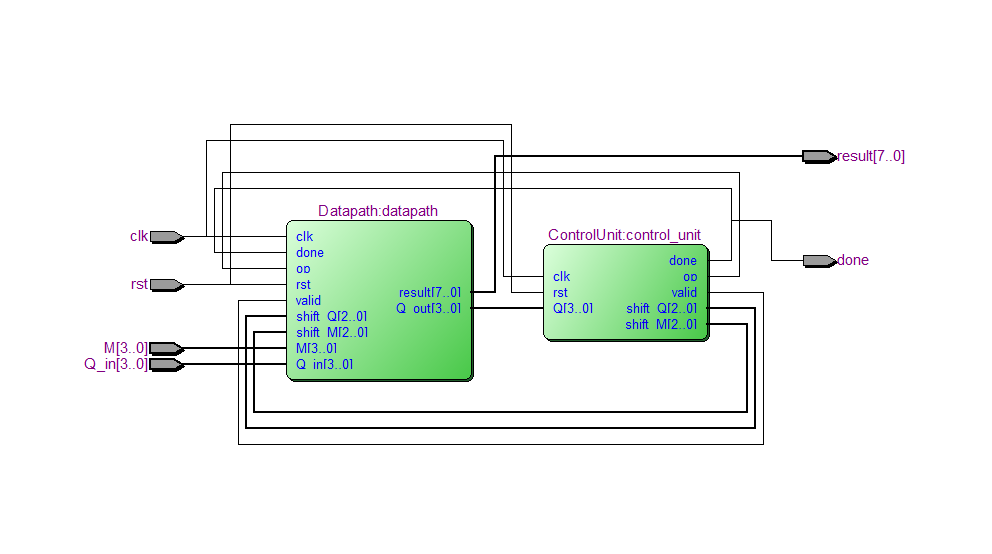
\includegraphics[width=1\textwidth]{images/rtl_viewer.png}
    \caption{نمای سطح انتقال ثبات (\lr{RTL Viewer})}
\end{figure}

\begin{figure}[H]
    \centering
    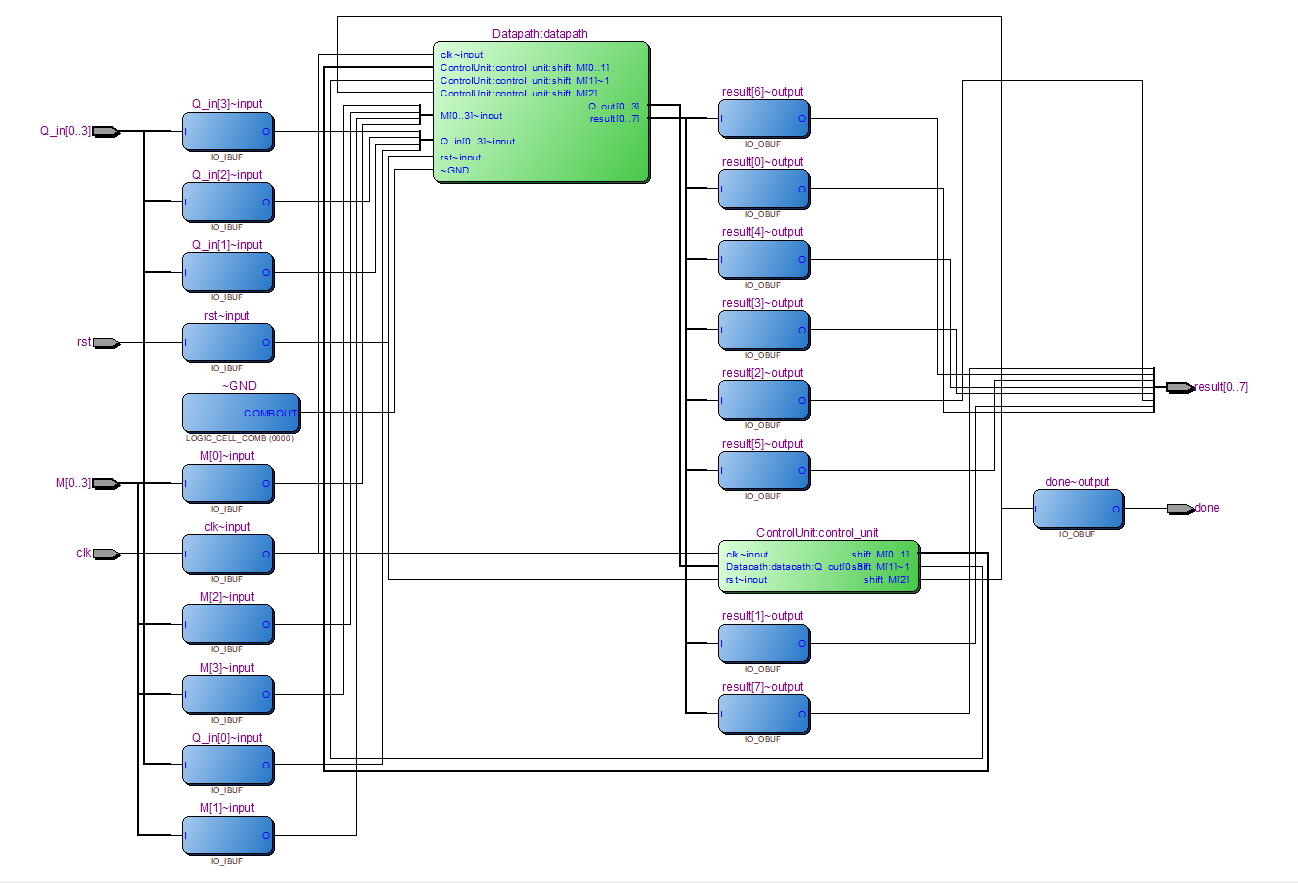
\includegraphics[width=1\textwidth]{images/tech_map_post_mapping.png}
    \caption{نمای نگاشت فناوری پس از نگاشت (\lr{Post-Mapping})}
\end{figure}

\begin{figure}[H]
    \centering
    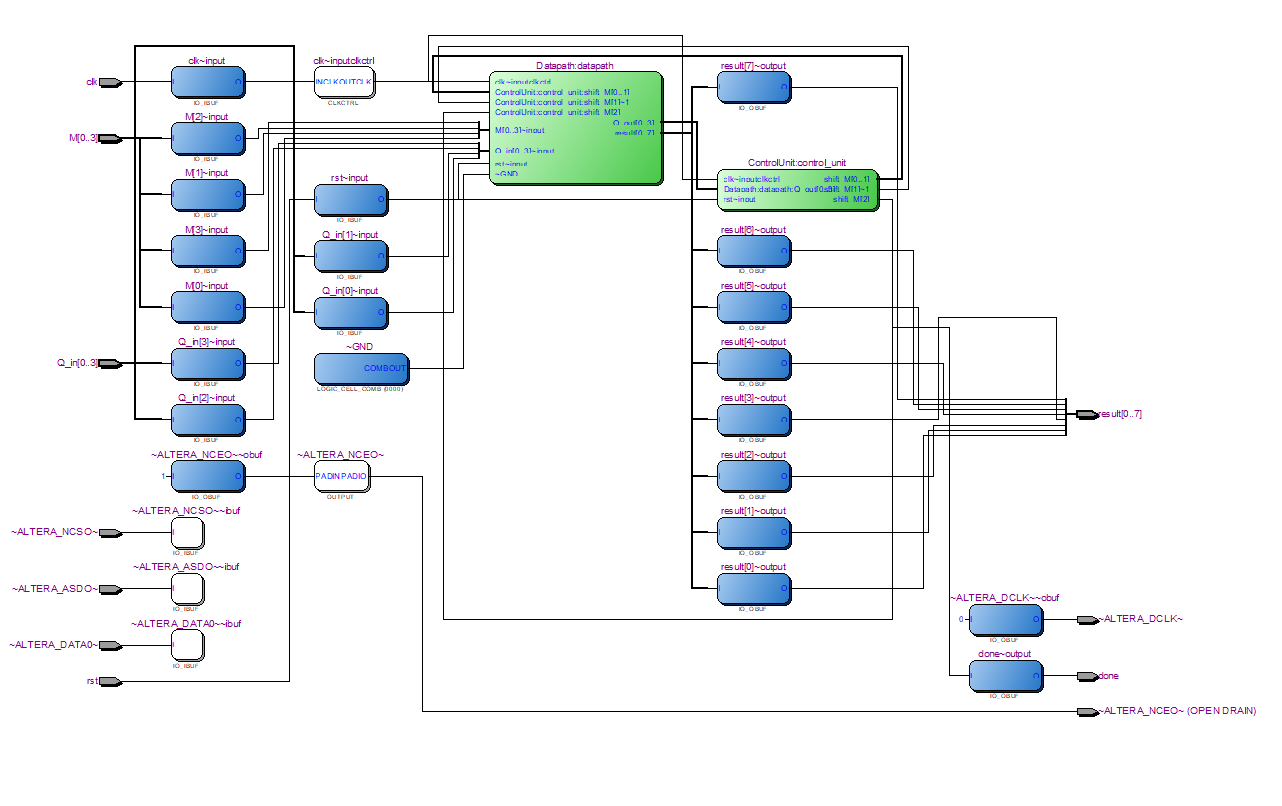
\includegraphics[width=1\textwidth]{images/tech_map_post_fitting.png}
    \caption{نمای نگاشت فناوری پس از جایابی و تطبیق (\lr{Post-Fitting})}
\end{figure}

\end{document}